{\tabulinesep=1mm
\begin{tabu}{|p{16cm} |}
\hline
Now instead of losing packets, we know that $k$ packets are corrupted. 
Furthermore, we do not know which $k$ packets are changed. Instead of 
sending $k$ additional packets, we will send an additional $2k$.\newline
\begin{center}

\includegraphics[width=8cm, height=0.6cm]{general_intro.jpg}
\end{center}

\textbf{Solomon-Reed Codes}
\begin{enumerate}
\item Identical to erasure errors: Alice creates $n - 1$ degree polynomial 
$P(x)$.\newline
\[P(x) = p_0 + p_1x + \dotsc + p_{n-1}x^{n-1} \]
\item Alice sends $P(1), \dotsc, P(n + 2k)$ \\
\item Bob receives $R(1), \dotsc, R(n + 2k) $ \newline
\end{enumerate}

For how many points does $R(x) = P(x)$? \newline
\begin{solution}
$ n + k$
\end{solution}

True or false: $P(x)$ is the unique degree $n - 1$ polynomial that goes 
through at least $n + k$ of the received points.\newline
\begin{solution}
True
\end{solution}

Write the matrix view of encoding the points $P(1), \dotsc, P(n + 2k)$
\begin{solution}[1cm]
\begin{center}
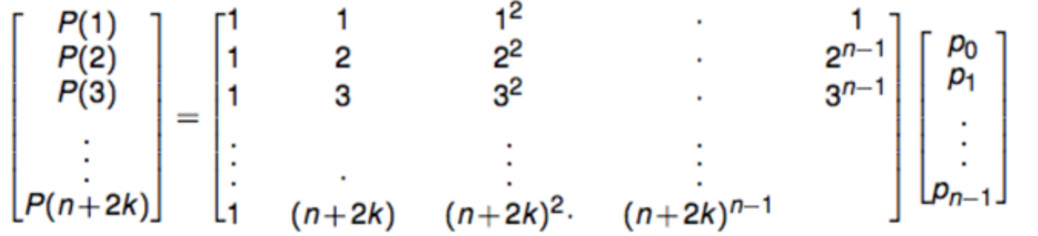
\includegraphics[width=9cm, height=2.3cm]{general_intro_matrix.jpg}
\end{center}
\end{solution}

\\
\hline
\end{tabu}
}

\clearpage
{\tabulinesep=1mm
\begin{tabu}{|p{16cm} |}
\hline
\textbf{Berlekamp Welch} \newline
How do we find the original polynomial $P(x)$? \newline
Suppose that $m_1, \dotsc, m_k$ are the corrupted packets. Let $E(x) = (x - m_1) \dotsc (x - m_k)$
Then $P(i) * E(i) = r_i * E(i)$ for any $i$ greater than 1 and less than $n + 2k$. Why?
\begin{solution}[5 cm]
	Case 1: $i$ is corrupted
\[E(i) = 0 \rightarrow 0 = 0\]
			Case 2: $i$ is not corrupted
				\[P(i) = r_i \rightarrow P(i) * E(i) = r_i E(i)\]
\end{solution}

Let $Q(i) = P(i) E(i)$
So we have $Q(i)= P(i) E(i) = r_i * E(i)$ where $1 \leq i \leq 2k + n$
What degree is $Q(i)$? 
\begin{solution}[1 cm]
$n + k - 1$
\end{solution}

How many coefficients do we need to describe $Q(i)$? 
\begin{solution}[1 cm]
$n + k$
\end{solution}

What degree is $P(i)$? 
\begin{solution}[1 cm]
$n - 1$
\end{solution}

How many unknown coefficients do we need to describe $E(i)$? 
\begin{solution}[2 cm]
$k$ (we know that the first coefficient has to be 1)
\end{solution}

We can write $Q(i) = r_i E(i)$ for every $ i$ that is $1 \leq i \leq 2k + n$. \newline
How many equations do we have? How many unknowns? 
\begin{solution}[1 cm]
$n + 2k$
\end{solution}

Once we have the above described equations, how do we determine what 
$P(i)$ is?
\begin{solution}[3 cm]
Solve the equations to get the coefficients for $E(i)$ and $Q(i)$. 
Then divide $\frac{Q(i)}{E(i)}$ to get $P(i)$.
\end{solution}
\\
\hline
\end{tabu}
}
